\documentclass[12pt]{article}
\usepackage{amsmath}
\usepackage{graphicx}
\usepackage{adjustbox}
\usepackage{booktabs}
\usepackage{tabularx}
\usepackage{fullpage}
\usepackage{subcaption}
\usepackage{cite}
\usepackage{float} % Added to allow [H] float specifier



\title{Cross-Indicator Prediction of Major Economic Indicators}
\author{Jiadong Zhang\thanks{Email: \texttt{dereksodo@gmail.com}}}
\date{May 2025}

\begin{document}

\maketitle

\begin{abstract}
This study explores the predictability of major macroeconomic indicators using machine learning models. Starting from a cross-indicator prediction framework based on World Bank panel data (1960--2020), it extends to time series modeling for individual countries and cross-national forecasting for major economies. The results show that most structural indicators are highly predictable, while GDP growth remains challenging. The work provides a spatio-temporal framework for economic indicator prediction and highlights the role of different model types and data contexts.
\end{abstract}

\newpage
\tableofcontents
\newpage


\section{Introduction}

Macroeconomic indicators provide a comprehensive lens for assessing the economic and social development of countries. This study leverages World Bank panel data from 1960 to 2020 to identify key national indicators and evaluate their predictability using machine learning. The focus is on cross-indicator prediction: can one major indicator be reliably predicted from the others?
\section{Literature Review}

Recent advancements in machine learning (ML) have significantly influenced macroeconomic forecasting. This section reviews key studies that have explored the integration of ML techniques into economic prediction models.

\subsection{Nonlinearity and Regularization in ML Forecasting}

Goulet Coulombe et al. (2019) investigate the efficacy of ML in macroeconomic forecasting, emphasizing the importance of capturing nonlinear relationships in economic data. Their study concludes that nonlinearity is a crucial factor in improving forecast accuracy. They also highlight that traditional factor models serve as effective regularization tools within ML frameworks, aiding in managing model complexity and preventing overfitting. The authors advocate for the use of K-fold cross-validation as a best practice for model evaluation and selection. Their findings suggest that ML models, when properly regularized and validated, can outperform traditional econometric models, especially during periods of economic uncertainty and financial stress \cite{GouletCoulombe2019}.

\subsection{Automating Forecasting with ML Techniques}

Hall (2018) explores the application of ML methods to macroeconomic forecasting, focusing on the automation of model selection and parameter tuning. The study demonstrates that ML algorithms can process vast and complex datasets, identifying patterns that traditional models might overlook. Hall's analysis reveals that ML models can outperform both simple time-series models and consensus forecasts from professional economists, particularly in predicting short-term economic indicators like the unemployment rate. The research underscores the potential of ML to enhance forecasting accuracy by reducing reliance on manual model specification and expert judgment \cite{Hall2018}.

\subsection{ML Applications in China's GDP Forecasting}

Yang et al. (2024) apply various ML models to forecast China's quarterly real GDP growth, assessing their performance against traditional econometric models and expert forecasts. Their study finds that ML models generally achieve lower forecast errors, particularly during stable economic periods. However, during economic inflection points, expert forecasts may exhibit greater accuracy due to a more nuanced understanding of the macroeconomic environment. Additionally, the authors employ interpretable ML techniques to identify key variables influencing GDP fluctuations, providing insights into the underlying drivers of economic change \cite{Yang2024}.

\subsection{Synthesis and Implications for Current Research}

The reviewed studies collectively highlight the transformative impact of ML on macroeconomic forecasting. They demonstrate that ML models, with their ability to capture complex nonlinear relationships and process large datasets, can enhance forecast accuracy beyond traditional methods. These findings inform the current research by underscoring the importance of incorporating ML techniques into economic prediction models, particularly for analyzing cross-indicator relationships, time series data, and cross-country economic dynamics.


% This section should review key literature on macroeconomic forecasting using machine learning.
% Include comparisons of cross-indicator modeling, single-country time series forecasting, and international panel data approaches.
% Discuss how your work extends or differs from past studies such as Goulet Coulombe (2019), Hall (2018), and Yang et al. (2024).
\section{Data and Methods}

\subsection{Data Source}

\begin{itemize}
    \item World Bank Open Data, 1960--2020, including G20 expect African Union.
    \item Main dataset: [World Bank Data by Indicators](https://github.com/light-and-salt/World-Bank-Data-by-Indicators) (GitHub repository)
    \item We choose 40 features, 2 representative features each in 20 categories by the World Bank.\footnote{See src/utils.py/feature\_codes for 40 initial features}
Some data are missing, and we only choose features if more than 60\% of relevant data are present. After cleaning and imputation, Principal Component Analysis (PCA) was used to select 10 relatively independent indicators, denoted $\{F_1, F_2, \ldots, F_{10}\}$, each with a feature load denoting how well it can "predict" other indicators. \footnote{Check Table \ref{tab:indicator_table} for details.}
\end{itemize}

\begin{table}[H]
    \centering
    \small
    \adjustbox{center}{
        \begin{tabular}{|c|c|c|}
            \hline
            \textbf{Indicator Code} & \textbf{Indicator Name} & \textbf{Feature Loading} \\
            \hline
            SP.DYN.LE00.IN & Life expectancy at birth, total (years) & 0.36759578 \\
            SP.URB.TOTL.IN.ZS & Urban population (\% of total population) & 0.34436319 \\
            NV.AGR.TOTL.ZS & Agriculture, forestry, and fishing, value added (\% of GDP) & -0.34223186 \\
            EG.USE.PCAP.KG.OE & Energy use (kg of oil equivalent per capita) & 0.28370116 \\
            FS.AST.PRVT.GD.ZS & Assets of private sector banks to GDP (\%) & 0.22820370 \\
            NE.IMP.GNFS.ZS & Imports of goods and services (\% of GDP) & 0.19327803 \\
            NY.GDP.MKTP.CD & GDP (current US\$) & 0.18121013 \\
            NE.EXP.GNFS.ZS & Exports of goods and services (\% of GDP) & 0.16005320 \\
            NY.GDP.MKTP.KD.ZG & GDP growth (annual \%) & -0.12023558 \\
            EN.ATM.GHGT.KT.CE & Total greenhouse gas emissions (kt of CO$_2$  equivalent) & 0.08242521 \\
            \hline
        \end{tabular}
    }
    \caption{Indicator Table}
    \label{tab:indicator_table}
\end{table}



\subsection{Data Preprocessing}

\begin{itemize}
    \item Interpolated missing values for convenience.\footnote{See /src/feature\_engineering.py}
    \item Constructed a country-year-feature panel: each row is a unique (country, year) pair.
\end{itemize}
We have some explanations about this. Negative feature loadings in this context should be interpreted as showing the direction of contribution relative to other features, and they often reflect well-established economic phenomena—such as the declining share of agriculture in GDP with development, or the varying relationship between growth rates and structural economic factors.
The sign itself is not inherently meaningful on its own, but should be understood in the context of the overall model and dataset.

For “Agriculture, forestry, and fishing, value added (\% of GDP)”, a negative loading often reflects the empirical reality that, as countries develop, the relative contribution of agriculture to GDP typically decreases—even as the economy grows overall. In higher-income economies, agriculture forms a smaller percentage of total output. Thus, in a multivariate context, a negative loading may simply capture this pattern of structural transformation.

For “GDP growth (annual \%)”, a negative loading could indicate that, within the chosen principal component or regression direction, higher GDP growth rates are associated with lower values of the principal component or the target variable—perhaps due to cyclical effects, catch-up growth in developing economies, or statistical collinearity with other features in the dataset.





\subsection{Machine Learning Models}

The following models are compared\footnote{See /src/models.py for parameters}:
\begin{itemize}
    \item Linear Regression (LR)
    \item Ridge Regression
    \item Lasso Regression
    \item Elastic Net
    \item Support Vector Regression (SVR)
    \item Random Forest (RF)
    \item K-Nearest Neighbors (KNN)
    \item XGBoost
    \item Locally Weighted Regression (LWR)
\end{itemize}

\subsection{Experimental Setup}

\begin{itemize}
    \item \textbf{Year ranges:}
    \begin{itemize}
        \item Full period: 1960--2020
        \item Recent period: 2010--2020
    \end{itemize}
    \item \textbf{Cross-Validation:} 5-fold cross-validation is used for each prediction, averaging metrics across folds.
    \item \textbf{Evaluation Metrics:}
    \begin{itemize}
        \item Standardized error (RMSE/STD)
        \item Coefficient of Determination ($R^2$)
        \item Mean Absolute Scaled Error (MASE)
        \item Directional Accuracy (DA)
        \item \textbf{Feasibility Rate (Heuristic Indicator):} For each model and indicator, we define a feasibility score as the average proportion of cases where at least 3 out of 4 predictions fall within an acceptable region. Specifically, we compute:
        \begin{align*}
        \alpha_1 &= \mathbf{1}\left[\frac{\text{RMSE}_i}{\text{STD}_i} < 1\right] \\\\
        \alpha_2 &= \mathbf{1}\left[R_i^2 > 0.6\right] \\\\
        \alpha_3 &= \mathbf{1}\left[\text{MASE}_i < 1\right] \\\\
        \alpha_4 &= \mathbf{1}\left[\text{DA}_i > 0.7\right]
        \end{align*}
        \[
        \text{Feasibility Rate} = \frac{1}{N} \sum_{i=1}^N \mathbf{1}\left[ \sum_{j=1}^4 \alpha_i \geq 3\right]
        \]
        This indicator serves as a summary of how often a model’s predictions are statistically reliable according to our predefined thresholds.
    \end{itemize}
    \item \textbf{Visualization:} For each model and year range, bar plots of the 4 metrics are generated, with feasible region thresholds indicated.
\end{itemize}

\section{Cross-Indicator Analysis}

\subsection{Prediction Task}
For each indicator $F_k$, we predict its value for each country-year using the remaining 9 indicators as input features. The process is repeated for all $k = 1, \ldots, 10$.
\subsection{Prediction Results}
% Retain your current performance evaluation here.

% Sample Figure Placeholders
\begin{figure}[h]
    \centering
    \begin{subfigure}[b]{0.48\textwidth}
        \centering
        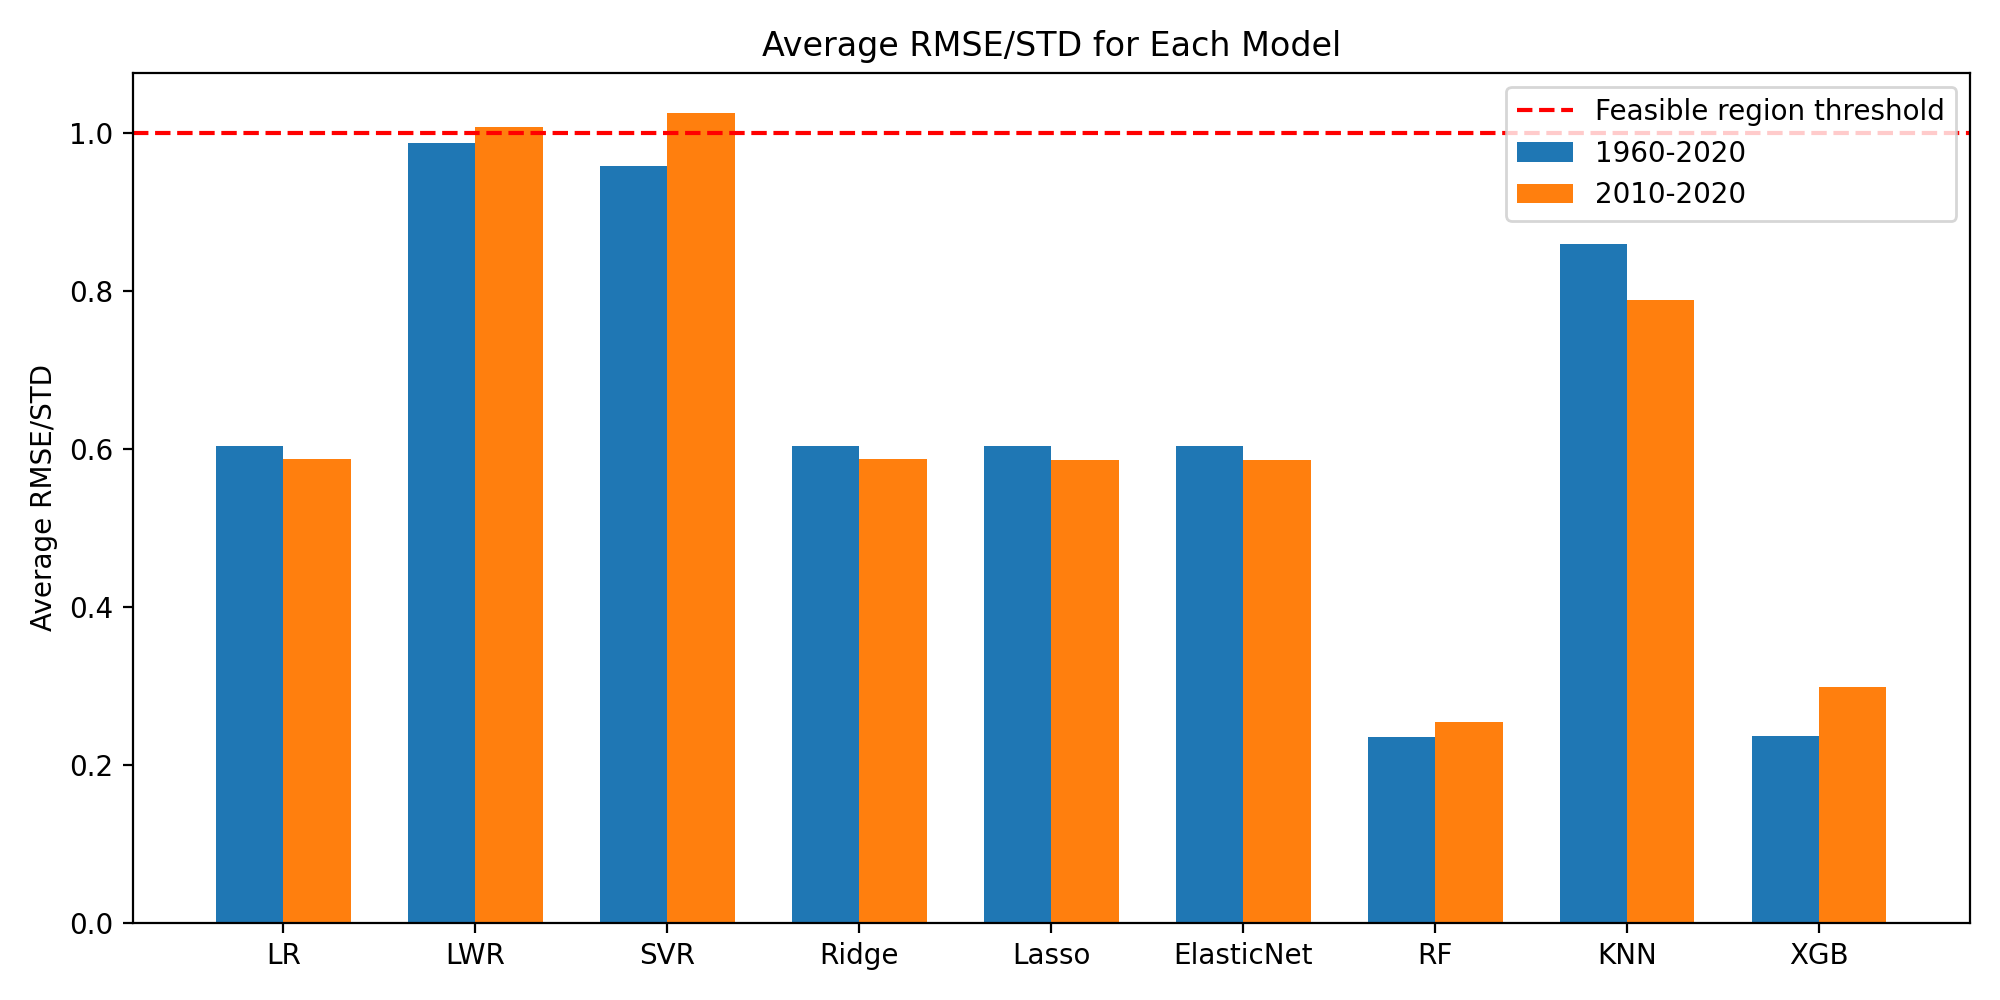
\includegraphics[width=\linewidth]{Average_RMSE_STD_figure1.png}
        \label{fig:rmse_std}
    \end{subfigure}
    \hfill
    \begin{subfigure}[b]{0.48\textwidth}
        \centering
        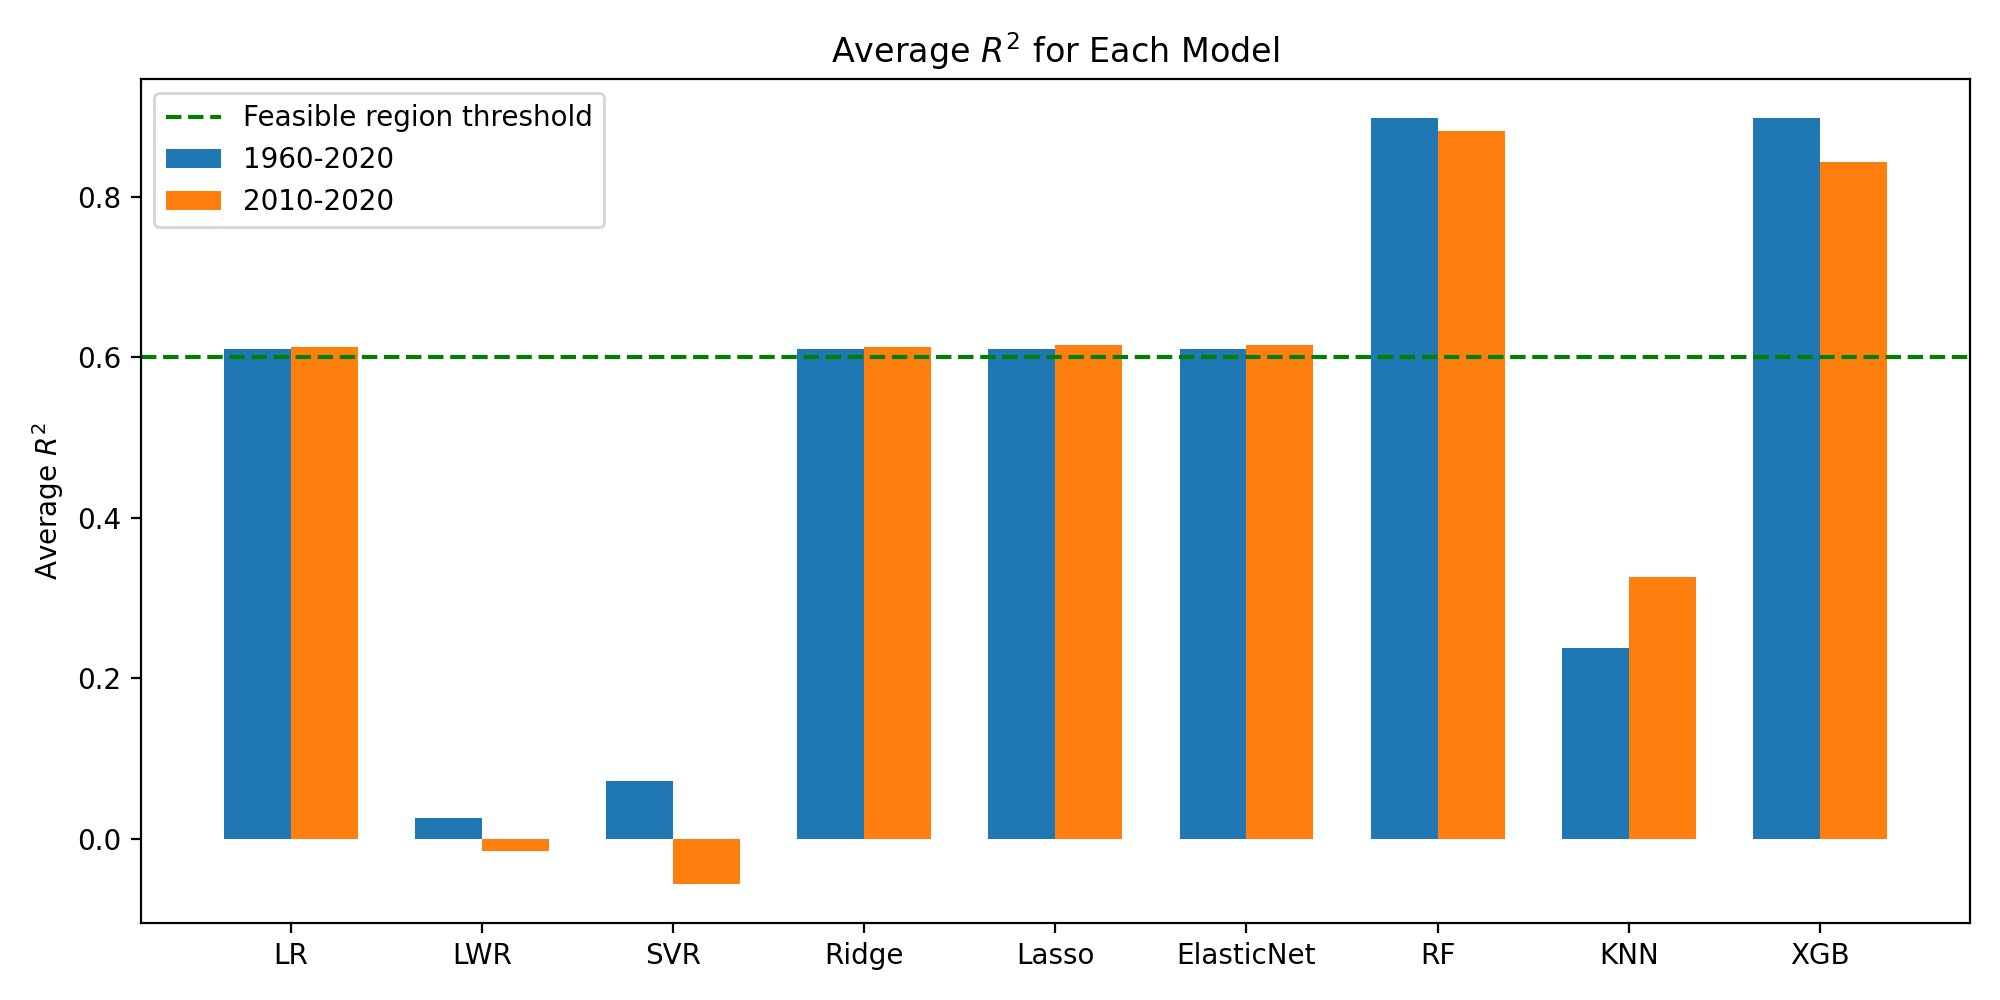
\includegraphics[width=\linewidth]{Average_R2_figure1.png}
        \label{fig:r2}
    \end{subfigure}
    \caption{Comparison of Model Performance: RMSE/STD and $R^2$ (1960–2020, 2010–2020)}
    \label{fig:model_compare_1}
\end{figure}
\begin{figure}[h]
    \centering
    \begin{subfigure}[b]{0.48\textwidth}
        \centering
        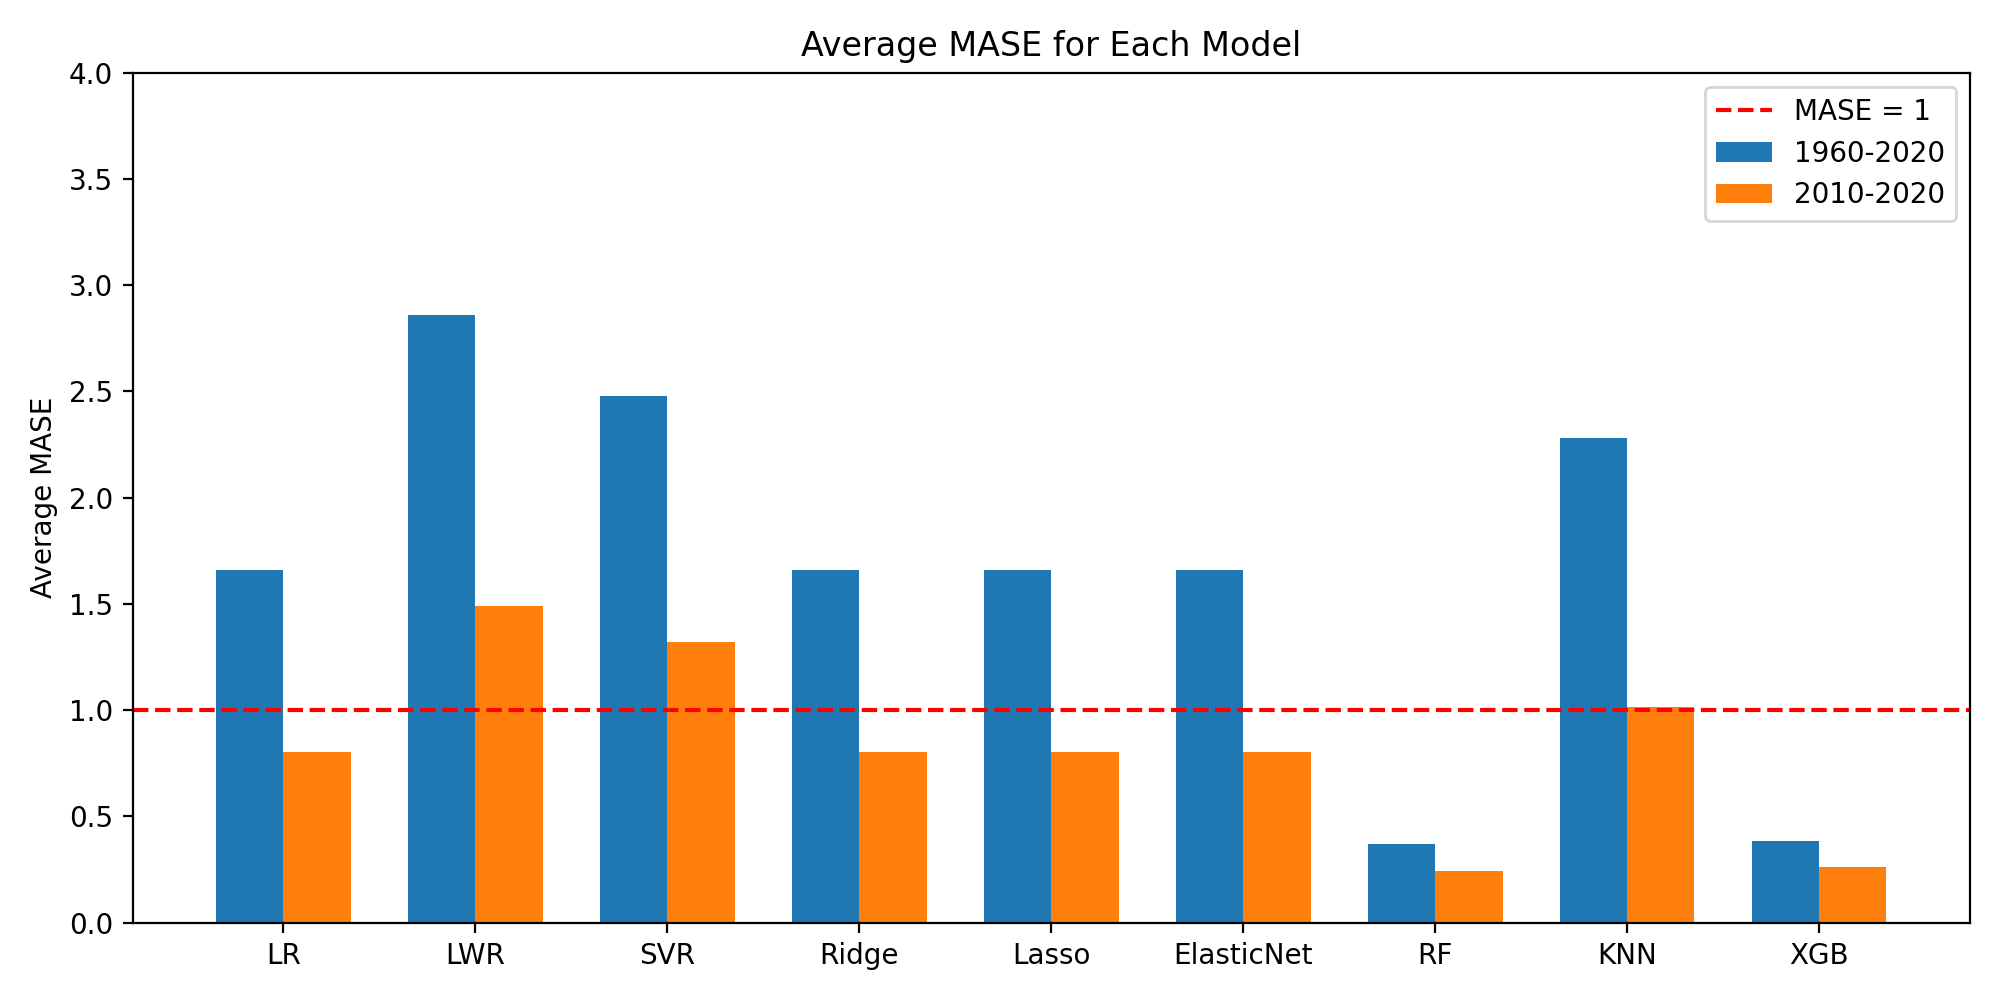
\includegraphics[width=\linewidth]{Average_MASE_figure2.png}
        \label{fig:MASE}
    \end{subfigure}
    \hfill
    \begin{subfigure}[b]{0.48\textwidth}
        \centering
        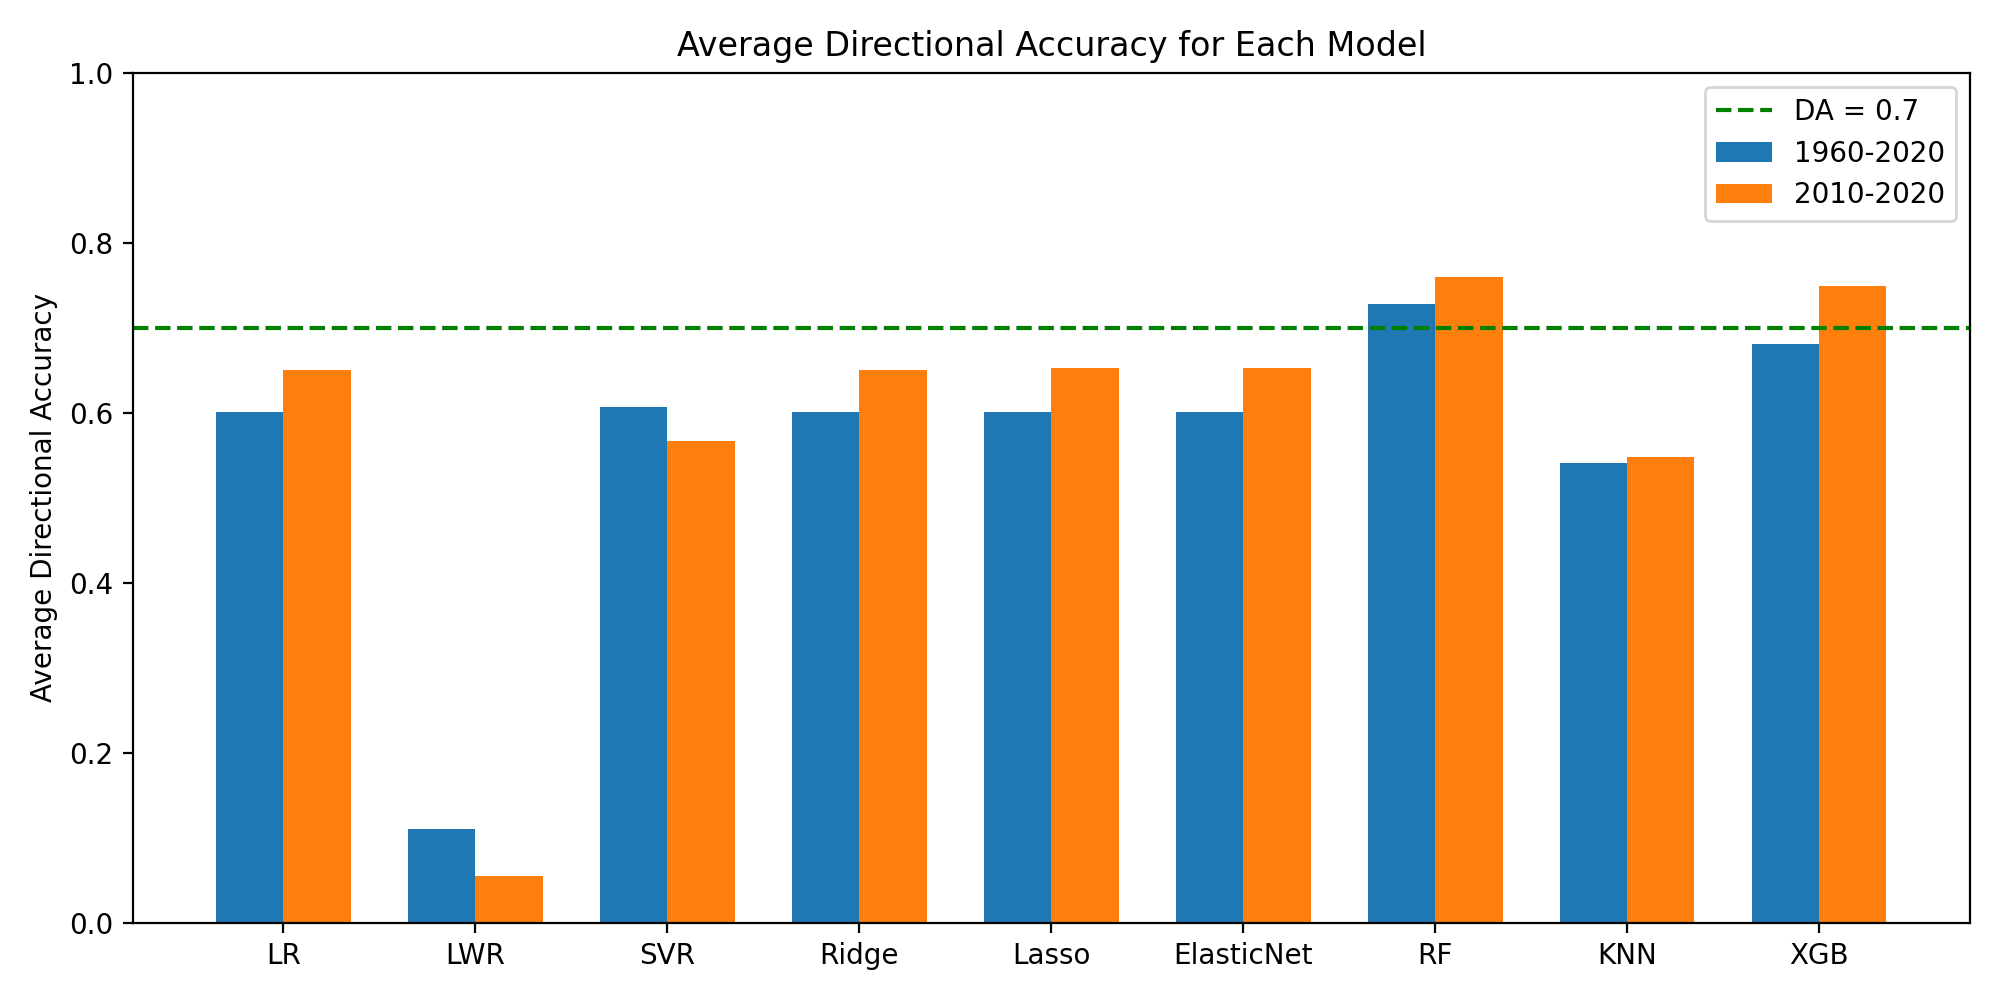
\includegraphics[width=\linewidth]{Average_DA_figure2.png}
        \label{fig:DA}
    \end{subfigure}
    \caption{Comparison of Model Performance: MASE and DA (1960–2020, 2010–2020)}
    \label{fig:model_compare_2}
\end{figure}
\begin{figure}[h]
    \centering
    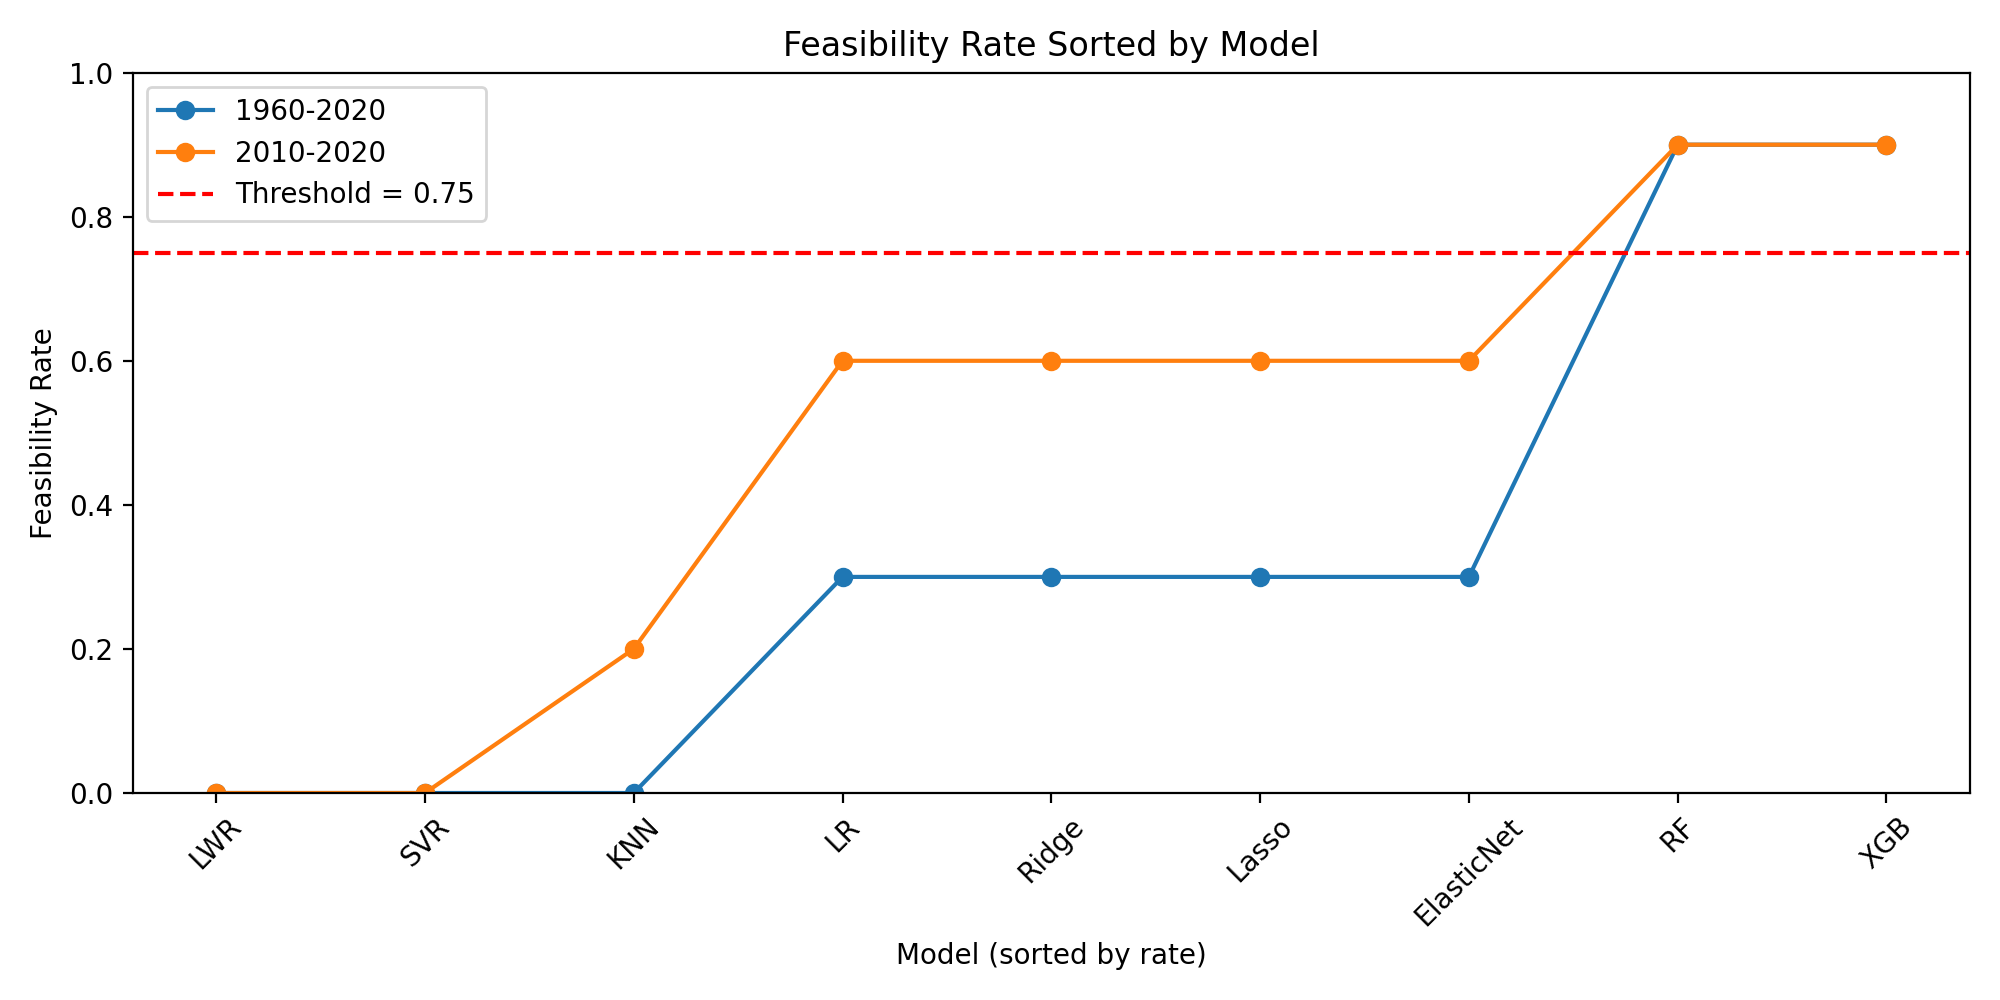
\includegraphics[width=0.8\linewidth]{Feasibility_Rate_Line_Overlay_figure3.png}
    \caption{Feasibility Rate comparison across models in different periods}
    \label{fig:FR}
\end{figure}



We can divide these Machine Learning algorithms into 3 different categories: 
\begin{itemize}
\item RF and XGB have best performances, both of which has a low standardized error, MASE and high $R^2$ and DA, with a feasibility rate of 0.95
\item LR, Ridge, Lasso, ElasticNet have very similar performances, with a feasibility rate of 0.6 (2010-2020) or 0.3 (1960-2020)
\item LWR, SVR, KNN have comparatively low performances. This is in part because the sample size (M = 1220 or 220) is rather small compared to input features (N = 10)
\end{itemize}

\begin{figure}[h]
    \centering
    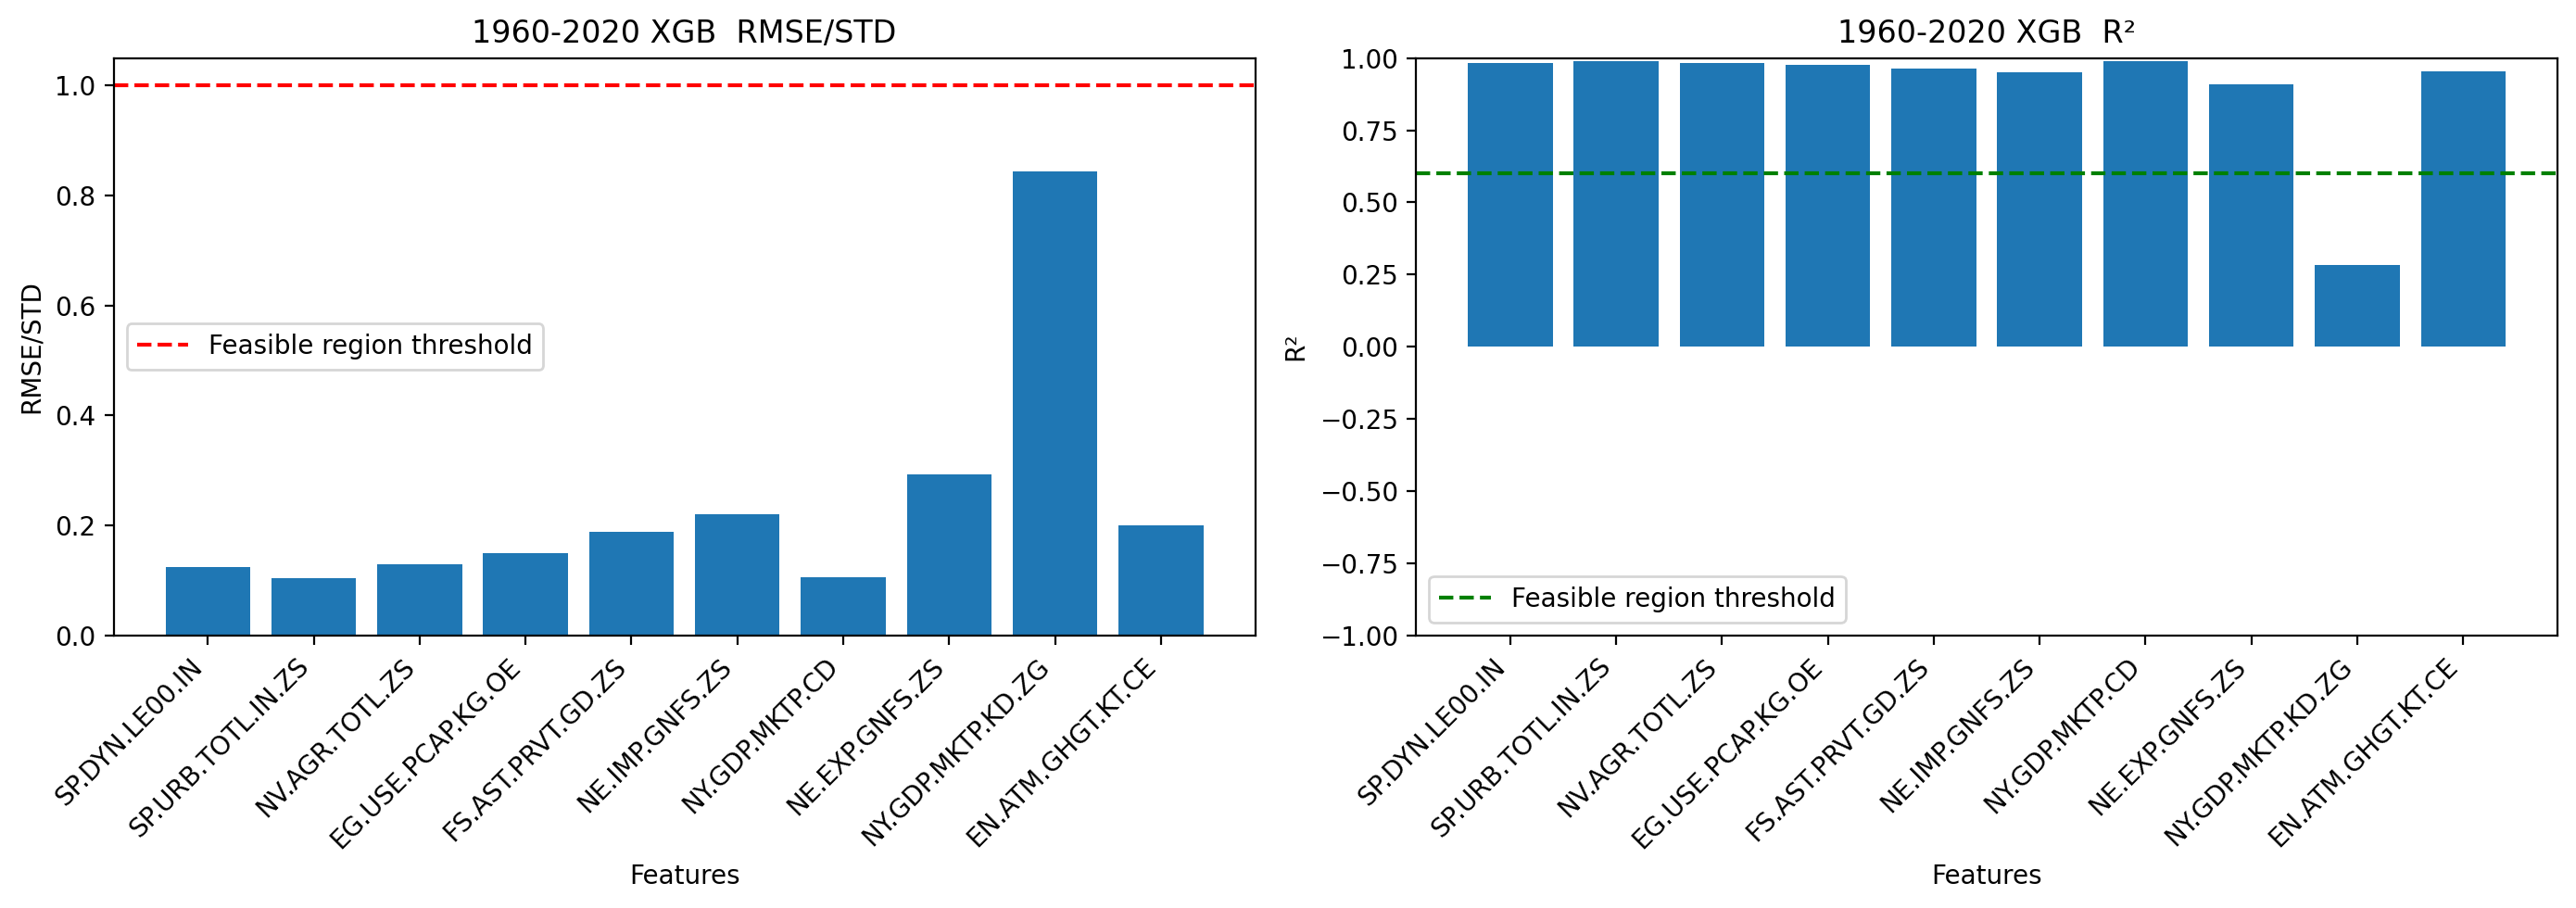
\includegraphics[width=0.95\textwidth]{1960_2020_XGB.png}
    
    \vspace{1em}  % 两图之间的垂直间距

    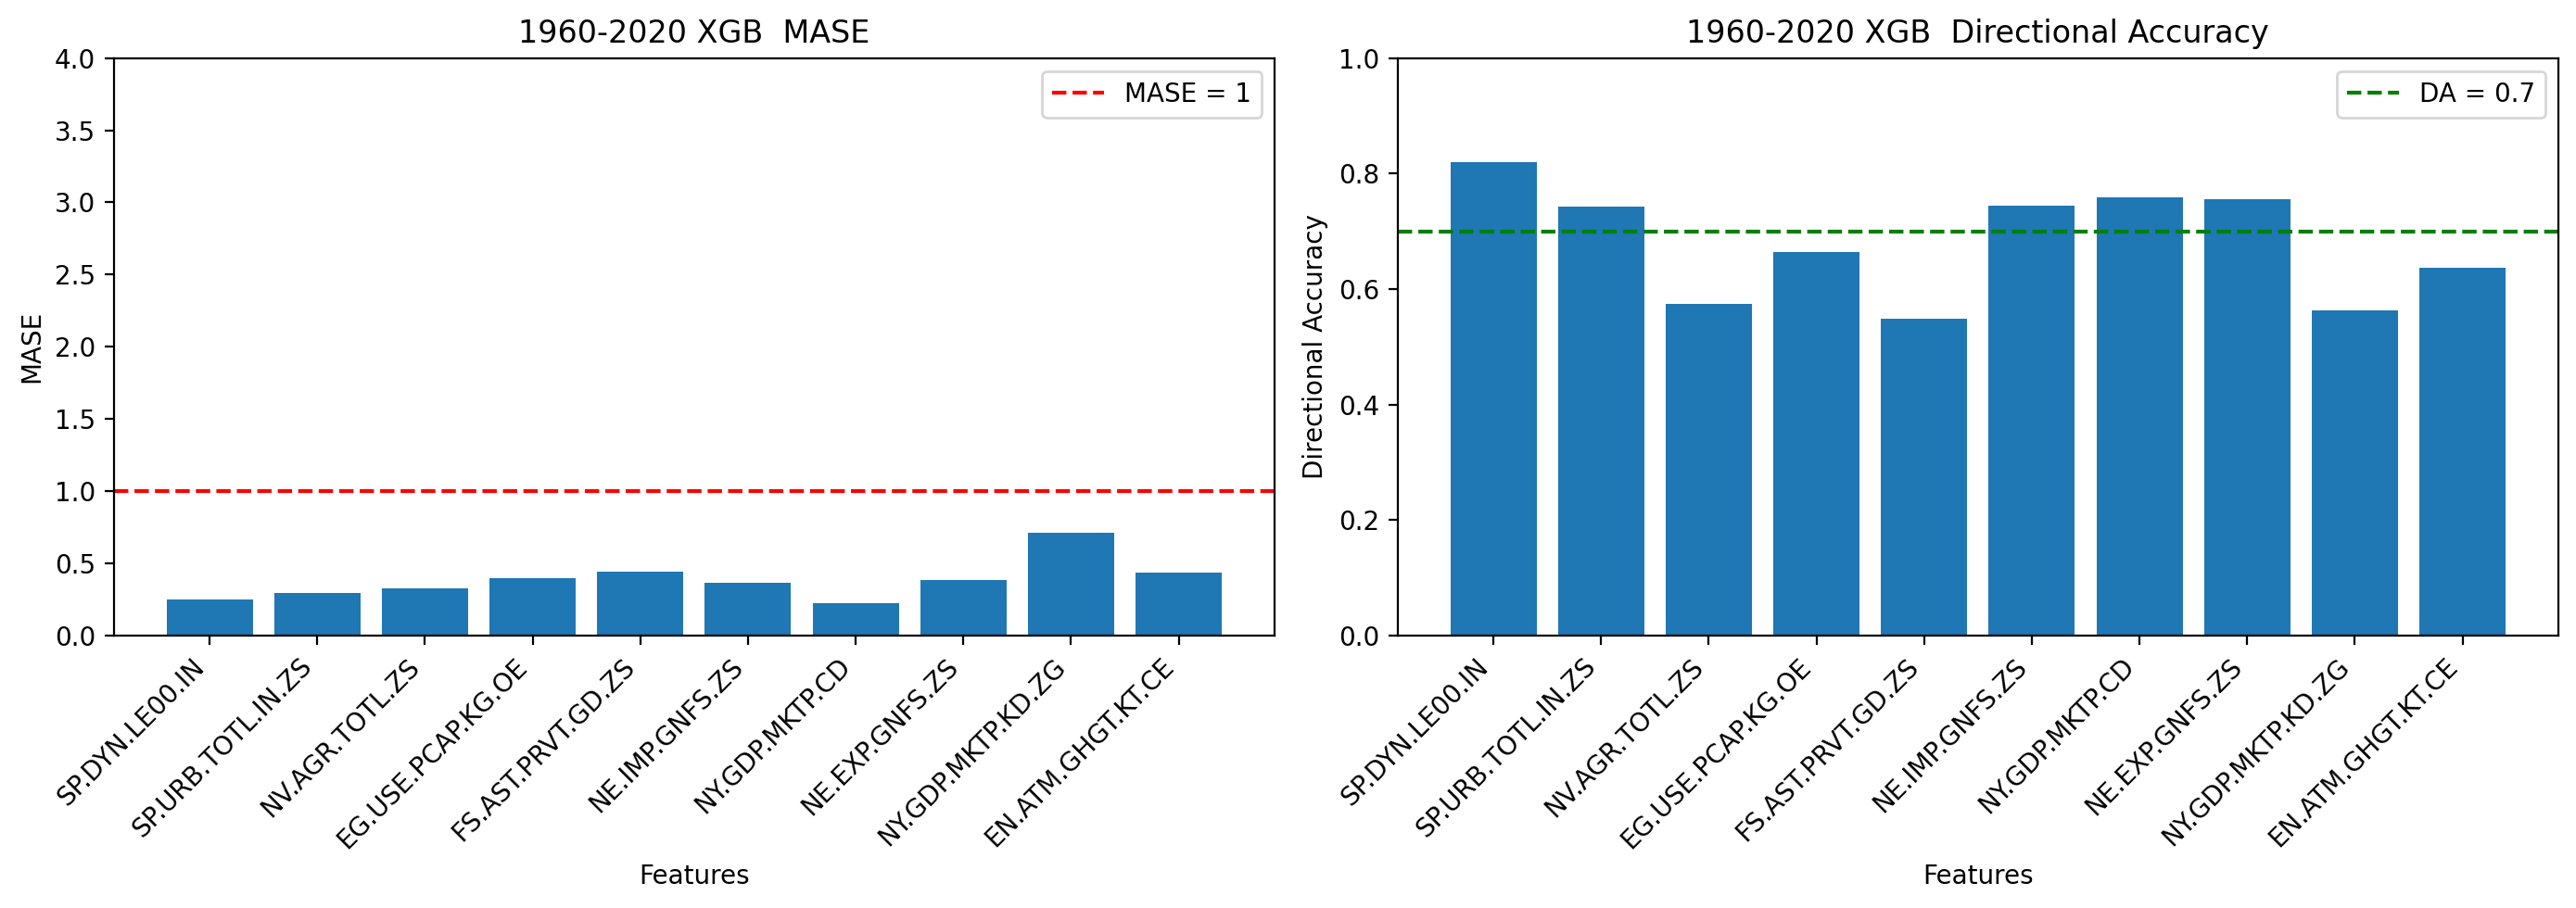
\includegraphics[width=0.95\textwidth]{1960_2020_XGB_mase_da.png}
    
    \caption{Prediction performance of XGBoost for each feature (1960--2020), including RMSE/STD, $R^2$, MASE, and Directional Accuracy.}
    \label{fig:xgb_feature_summary}
\end{figure}
Figure~\ref{fig:xgb_feature_summary} summarizes the prediction performance of XGBoost for each of the 10 selected indicators over the full period (1960--2020). The results indicate that XGBoost achieves high accuracy for most structural indicators, with standardized errors (RMSE/STD) well below 1 and $R^2$ values typically above 0.6. Notably, indicators such as life expectancy, urban population share, and energy use are predicted with particularly high precision. In contrast, GDP growth (annual \%) stands out as the only indicator with consistently poor predictive performance, exhibiting both high error and low explanatory power. The poor predictability of the GDP growth rate compared to other major indicators is primarily due to its intrinsic volatility, exposure to a broad set of unobserved influences, and its weak contemporaneous linkages with slow-moving structural features. This is a well-documented phenomenon in economic modeling ~\cite{Loungani2001, ClementsHendry2002}, where forecasting economic growth remains an exceptionally challenging task.

\subsection{Discussion}
% Discuss the observed performance differences and their economic interpretation.

In this part, we systematically evaluated the cross-predictability of major national indicators using a suite of machine learning algorithms on World Bank panel data spanning six decades. The evaluation leverages four complementary metrics—RMSE/STD, $R^2$, Mean Absolute Scaled Error (MASE), and Directional Accuracy (DA)—along with a composite feasibility rate that captures overall reliability across these dimensions.

Ensemble models such as Random Forest (RF) and XGBoost (XGB) exhibit consistently strong performance across all metrics and both time periods. Their feasibility rates remain the highest among all models, typically exceeding 0.9, reflecting their robustness in capturing complex, nonlinear structures in macroeconomic data.

Support Vector Regression (SVR) and Locally Weighted Regression (LWR), although still the least performant models overall, also show improvements in the recent decade. Their feasibility rates, while remaining low, increase relative to the 1960–2020 baseline, indicating that even the least effective models benefit from more recent data.

Crucially, all ten models exhibit improved performance in the 2010–2020 period. This universal improvement suggests that the recent decade offers more learnable patterns for predictive models. Several factors may explain this across-the-board enhancement. First, the 2010s saw improvements in global statistical infrastructure and data quality, resulting in fewer missing values and more reliable measurements~\cite{jerven2013poor}. Second, structural convergence across economies due to globalization likely increased feature similarity between countries, enhancing cross-national generalizability~\cite{baldwin2016great}. Third, post-crisis macroeconomic policy harmonization and greater institutional stability may have led to more stable, linearizable relationships among indicators~\cite{blanchard2015inflation}.

Nonetheless, GDP growth remains the only indicator that no model predicts with high reliability. Its feasibility remains low in both periods, consistent with prior findings that economic growth is inherently volatile and poorly explained by structural contemporaneous variables~\cite{ClementsHendry2002, Loungani2001}.

The feasibility rate offers a valuable heuristic summary of model reliability. By integrating binary thresholds across RMSE/STD, $R^2$, MASE, and DA, it allows for intuitive comparison of how frequently each model yields statistically acceptable forecasts across multiple indicators and periods.

In summary, the results emphasize not only the superiority of ensemble methods, but also the significant influence of data context: all models—even the weakest—became more effective when trained on recent, high-quality economic data. This highlights the dual importance of methodological choice and temporal data conditions in macroeconomic prediction.

\subsection{Hyperparameter Tuning for XGBoost and Random Forest}

To ensure robust performance from the ensemble models, we conducted hyperparameter tuning for both XGBoost (XGB) and Random Forest (RF) using grid search with 5-fold cross-validation.

For XGBoost, the primary hyperparameters adjusted include:
\begin{itemize}
    \item \texttt{n\_estimators}: Number of boosting rounds.
    \item \texttt{max\_depth}: Maximum depth of each tree.
    \item \texttt{learning\_rate}: Step size shrinkage used in updates.
    \item \texttt{subsample}: Fraction of observations to be randomly sampled for each tree.
    \item \texttt{colsample\_bytree}: Fraction of columns to be randomly sampled for each tree.
\end{itemize}

For Random Forest, the tuning focused on:
\begin{itemize}
    \item \texttt{n\_estimators}: Number of trees in the forest.
    \item \texttt{max\_depth}: Maximum depth of the tree.
    \item \texttt{min\_samples\_split}: Minimum number of samples required to split an internal node.
    \item \texttt{max\_features}: Number of features to consider when looking for the best split.
\end{itemize}

The tuning process selected the best combination of parameters based on cross-validated performance using the feasibility rate as the guiding metric. These optimized settings contributed to the consistent top-tier performance observed in 1960–2020 evaluation.
In addition to tuning global models for each algorithm, we extended the grid search process to each individual indicator. For every target variable, the model was trained and evaluated under multiple parameter combinations, allowing us to select an indicator-specific optimal configuration. \begin{figure}[H]
    \centering
    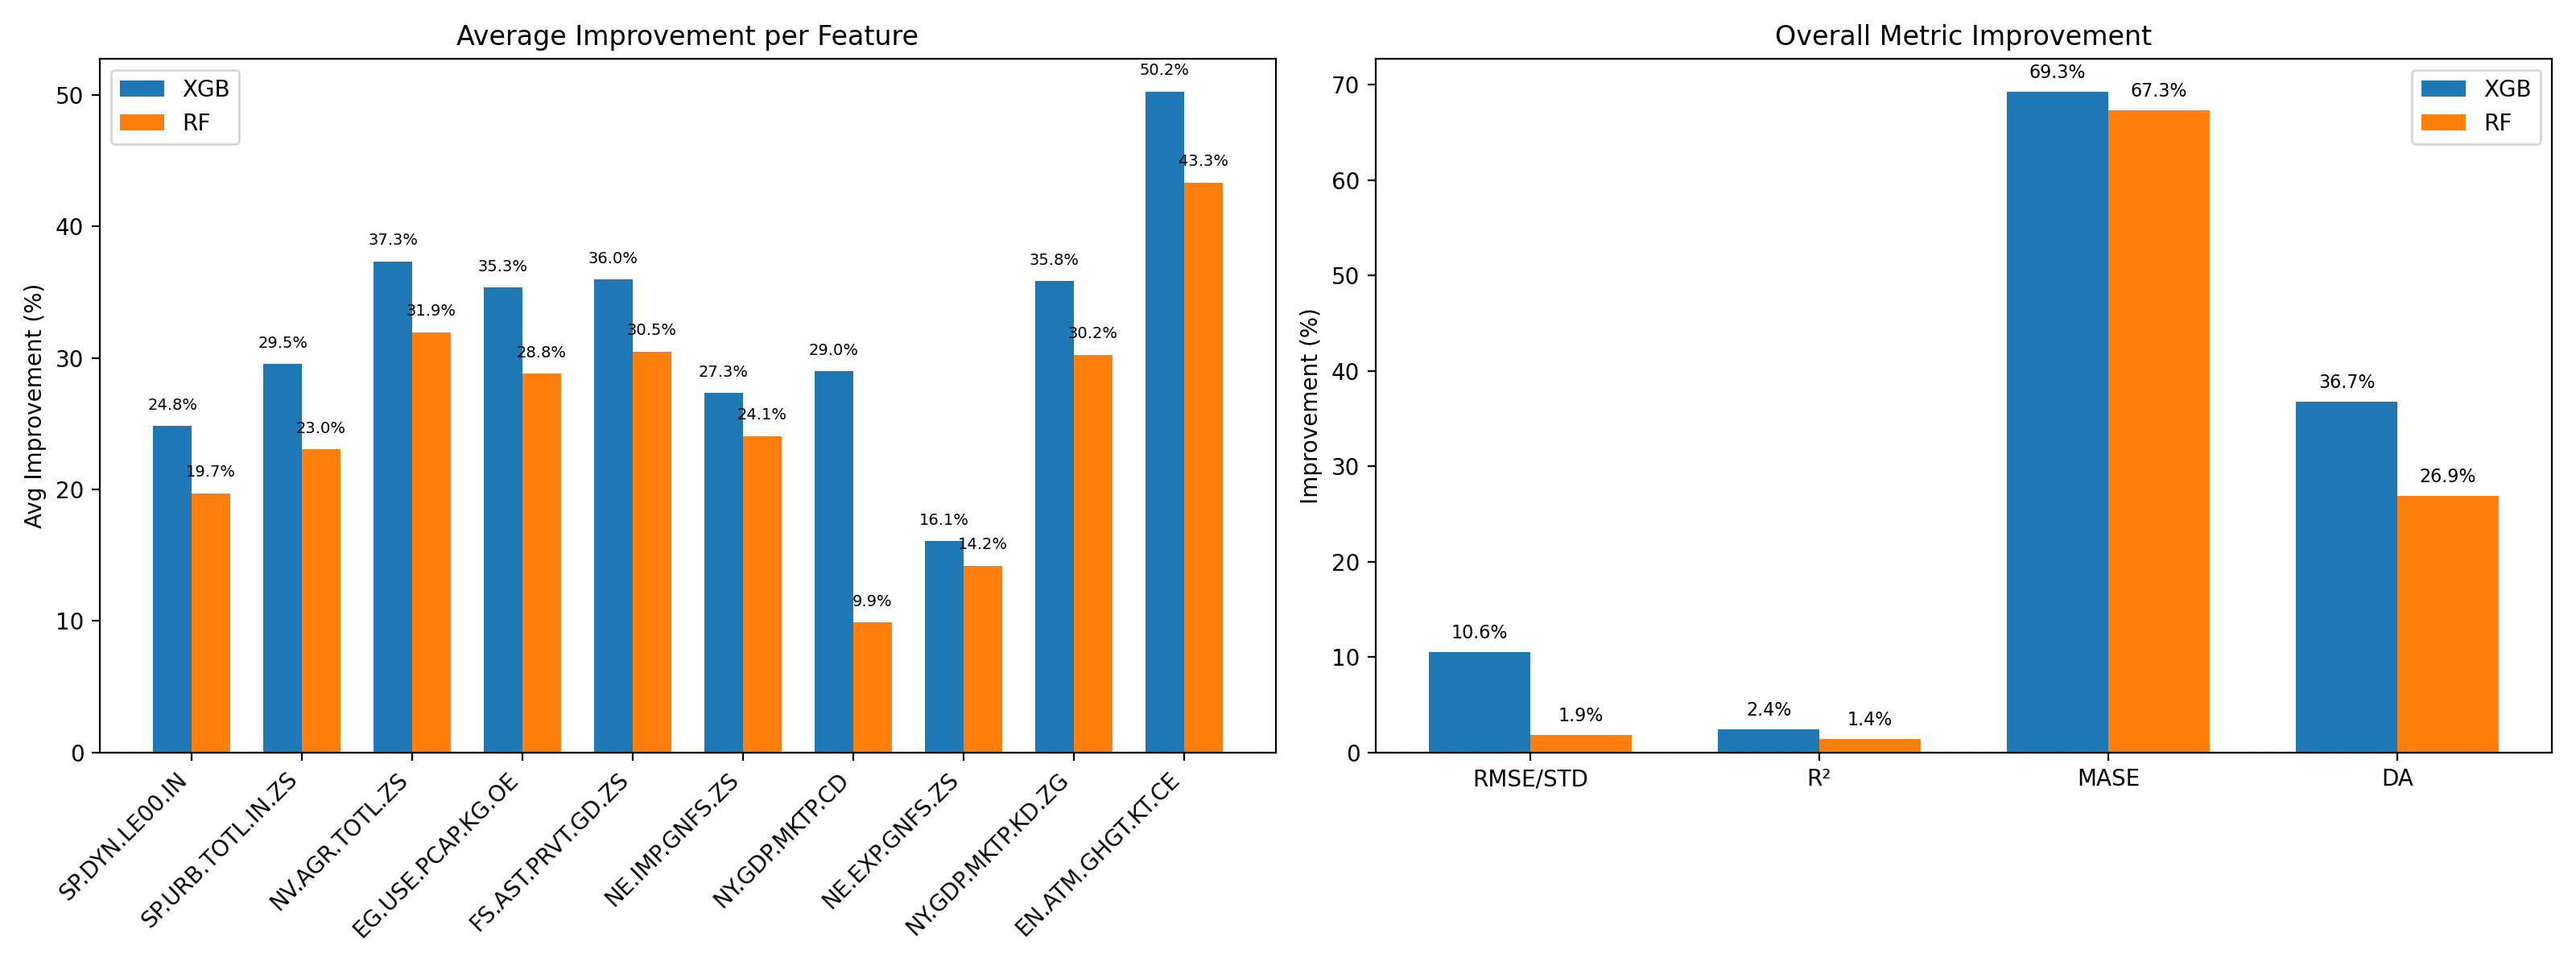
\includegraphics[width=\textwidth]{featurewise_and_modelwise_improvement.png}
    \caption{Feature-wise and overall metric improvement from hyperparameter tuning for XGBoost and Random Forest.}
    \label{fig:tuning_combined}
\end{figure}

Figure~\ref{fig:tuning_combined} provides a detailed visualization of the performance improvements after tuning. The left panel illustrates that while the magnitude of improvement\footnote{Calculated as average of improvement rate of 4 metrics} varies across indicators, all ten features experience a substantial average enhancement, with XGBoost consistently outperforming Random Forest in every case. This confirms that tuning has universal benefit, though its effect size depends on feature characteristics.

The right panel decomposes improvements across the four evaluation metrics. Notably, tuning yields minimal changes in $R^2$ (near 0\%), modest gains in RMSE/STD (ranging from 1\% to 10\%), and substantial improvements in Directional Accuracy (DA), which increase by approximately 30\%--40\%. The most dramatic effect is observed in Mean Absolute Scaled Error (MASE), where XGBoost and Random Forest achieves a nearly 70\% improvement. 
These results highlight how hyperparameter tuning differentially impacts specific model objectives and offer insights into which dimensions of forecast accuracy are most tunable.



\section{Country-Level Time Series Analysis}

\subsection{Temporal Feature Construction}
% Describe lag features, rolling means, or other temporal inputs created for each indicator at the national level.

\subsection{Forecasting Setup}
% Outline the task: predict F_k(t) using F_k(t-1), F_k(t-2), etc. Models may include ARIMA, XGBoost, or LSTM.

\subsection{Model Comparison}
% Compare forecasting performance of different time series models on a selected country.

\subsection{Case Study: [Insert Country]}
% Present RMSE, R², plots, and analysis of temporal predictability in that country.

\subsection{Discussion}
% Summarize which indicators are temporally predictable and why. Mention data density or volatility factors.

\section{Cross-Country Time Series Analysis}

\subsection{Selection of Major Economies}
% Specify which countries are analyzed (e.g., G7, BRICS).

\subsection{Modeling Setup}
% Define time alignment across countries. Optional: DTW similarity, cross-country lagged features.

\subsection{Cross-National Forecasting}
% Analyze how models trained on one or multiple countries generalize to others.

\subsection{Trend and Volatility Analysis}
% Identify persistent temporal trends vs high-volatility indicators across countries.

\subsection{Discussion}
% Reflect on structural similarity, transferable patterns, and policy relevance of findings.

\section{Conclusion}

This work demonstrates that most major structural indicators of national development are highly predictable from a small set of other key indicators, especially when using ensemble tree-based machine learning models. The exception is GDP growth rate, which remains notoriously difficult to forecast—consistent with macroeconomic theory and previous empirical research.

Our results suggest that, for long-run cross-country comparative analysis, reliable prediction of most economic and demographic indicators is feasible using standard machine learning approaches and open-access datasets. However, caution should be exercised when interpreting models for inherently volatile outcomes such as economic growth. Overall, this study highlights the promise and limitations of data-driven prediction in international development research and points to several avenues for further methodological and substantive refinement.


\section*{Project Repository}
The full code, data preprocessing scripts, and results can be found at: [GitHub link will be inserted here].



\bibliographystyle{unsrt}
\bibliography{references}
\end{document}